\section{Song aus Midi konvertieren}

Bisher haben wir manuell einen Song in einem Texteditor geschrieben. Für komplexere und längere Songs eignet sich das Konvertieren aus einer MIDI Datei. Ein Konverter übernimmt allerdings nur einen Teil unserer Arbeit. Die MIDI Datei muss vor dem Konvertiervorgang aufbereitet und das Ergebnis weiterhin im Texteditor bearbeitet werden.
\subsection{Vergleich der Konverter}
In diesem Kapitel werden drei Konverter vorgestellt, die alle Vor- und Nachteile mit sich bringen. Dabei handelt es sich um PetiteMM von gocha und loveemu, MIDI2MML von NeutronCat und mmltk von Nobody-86.
\subsubsection*{PetiteMM}
PetiteMM ist der mit Abstand älteste der drei Konverter mit einem simplen GUI.

\subsubsection*{Vorteile}
\begin{itemize}
	\item Java Programm lässt Benutzung auf Windows und MacOS zu
	\item Schneller Konvertiervorgang
	\item Konvertiert fast fehlerfrei
\end{itemize}

\subsubsection*{Nachteile}
\begin{itemize}
	\item Keine schöne MML Code Formatierung
\end{itemize}

\subsubsection*{MIDI2MML}
MIDI2MML ist ein neuerer Konverter aus Ende 2020.

\subsubsection*{Vorteile}
\begin{itemize}
	\item Benutzerfreundliches GUI
	\item Schneller Konvertiervorgang
	\item Schöne MML Code Formatierung
	\item Überlappende Noten werden über 8 Kanäle hinaus in separate Kanäle abgespeichert
	\item MIDI Events sind einsehbar
\end{itemize}

\subsubsection*{Nachteile}
\begin{itemize}
	\item C\# Programm, daher nur auf Windows zu benutzen
	\item Konverter interpretiert gewisse Notenwerte falsch
	\item Einige Notenwerte werden nicht intuitiv dargestellt.
\end{itemize}

\subsubsection*{mmltk}
mmltk ist ein weiterer neuerer Konverter aus Ende 2020, in Python geschrieben und als einziger Konsolenbasiert.

\subsubsection*{Vorteile}
\begin{itemize}
	\item Schöne MML Code Formatierung
	\item Überlappende Noten werden über 8 Kanäle hinaus in separate Kanäle abgespeichert
	\item Einziger Konverter der konstant fehlerfrei konvertiert
	\item Kann zusätzlich MML in eine MIDI Datei zurück konvertieren (experimentell)
\end{itemize}

\subsubsection*{Nachteile}
\begin{itemize}
	\item Programm momentan nur auf Windows zu benutzen
	\item Langsamer Konvertiervorgang
	\item Einmalige Installation aufwändiger als bei den anderen Konvertern
\end{itemize}

Da mmltk bei weitem das beste Ergebnis liefert, empfehle ich an dieser Stelle den einmaligen Mehraufwand der Installation.

\subsection{Installation und Benutzung von mmltk}
mmltk basiert auf Python, der erste Schritt ist also Python zu installieren.
Python kann hier heruntergeladen werden: \href{https://www.python.org/downloads/}{https://www.python.org/downloads/}

\bigskip

Als nächstes öffnen wir die Konsole und geben python -{}-version ein um zu testen, ob Python korrekt installiert wurde. Daraufhin sollte die Konsole mit der Versionsnummer von Python antworten.

\begin{figure}[htbp] \centering
	\includegraphics[width=.95\linewidth]{images/Python.png}
	\caption{Versionsnummer von Python aufrufen}
	\label{Python}
\end{figure}

mmltk benötigt 3 weitere Pakete die wir nun installieren und zwar mido, numpy und pandas.
Um die Pakete jeweils zu installieren, geben wir nacheinander

\bigskip

python -m pip install mido \\
python -m pip install numpy \\
python -m pip install pandas

\bigskip

ein. Ab jetzt können wir mmltk benutzen. Es kann unter \href{https://gitlab.com/Nobody-86/mmltk}{https://gitlab.com/Nobody-86/mmltk} heruntergeladen werden. \\
Nachdem wir die Datei an einem Ort unserer Wahl entpackt haben, öffnen wir wieder die Konsole.
Wir navigieren mit dem Befehl cd zu dem Verzeichnis, in dem mmltk.py liegt. Mit dem Befehl

\bigskip

python mmltk.py -i  \dq MIDINAME.mid\dq{} -o \dq MMLNAME.txt\dq{}

\bigskip

wird eine Midi in ein MML Dokument konvertiert, die im selben Verzeichnis liegt wie mmltk.py. \\
Alternativ kann auch der Pfad angegeben werden, falls die Midi nicht im selben Verzeichnis liegt wie mmltk.py. Tipp: Per Drag \& Drop wird automatisch der Dateipfad in die Konsole geschrieben.

\begin{figure}[htbp] \centering
	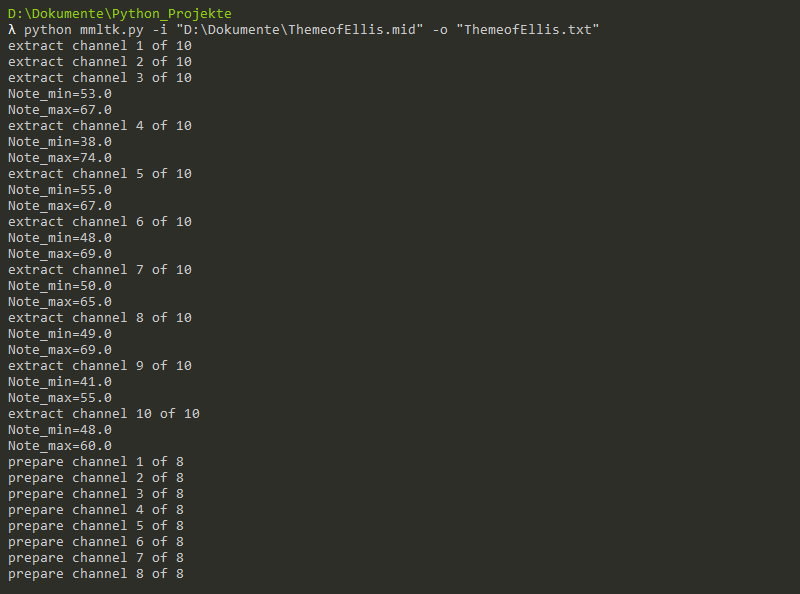
\includegraphics[width=.95\linewidth]{images/mmltk.png}
	\caption{MIDI mit mmltk in ein Textdokument mit MML konvertieren}
	\label{mmltk}
\end{figure}

\subsection{Midi aufbereiten und konvertieren}

Neben dem Konverter wird zusätzlich noch ein Programm benötigt, mit dem MIDIs (in einer Piano Roll) bearbeitet werden können. Beispiele dafür sind FL Studio, LMMS oder Anvil Studio. Die Trial Version von FL Studio reicht für unsere Zwecke vollkommen aus und beschränkt uns hinsichtlich des Arbeitens an Midi Dateien nicht. In diesem Tutorial benutze ich FL Studio und beschreibe den allgemeinen Umgang damit. \\
Wir öffnen eine beliebige MIDI Datei mit FL Studio, am einfachsten geht dies, indem die Datei per Drag \& Drop in das offene Programm gezogen wird. Wichtig hierbei ist, dass FL Studio nur MIDI Dateien mit der Endung .mid und nicht .midi öffnen kann. \\
Das folgende Fenster wird sich öffnen: 

\begin{figure}[htbp] \centering
	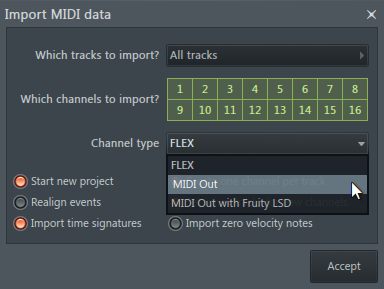
\includegraphics[width=.45\linewidth]{images/ImportMidi.png}
	\caption{MIDI mit FL Studio öffnen}
	\label{ImportMidi}
\end{figure}

Wir stellen den Channel type auf \textit{MIDI Out}. Falls zur MIDI Datei eine Soundbank in Form einer DLS (Downloadable Sound) Datei vorliegt, kann auch \textit{MIDI Out with Fruity LSD} ausgewählt werden. \textit{FLEX} sollte vermieden werden, besonders wenn man nur die Trial Version besitzt und keine FL Studio Projekte öffnen kann. FLEX Kanäle können notfalls auch im Nachhinein noch durch MIDI Out Kanäle ersetzt werden. \\
Als nächstes muss der MIDI Port geändert werden und zwar auf den gleichen, den auch die MIDI Out Kanäle verwenden (standardmäßig auf 0) Mit F10 öffnen sich die MIDI Settings, dort stellen wir den Port auf 0.

\bigskip

\begin{figure}[htbp] \centering
	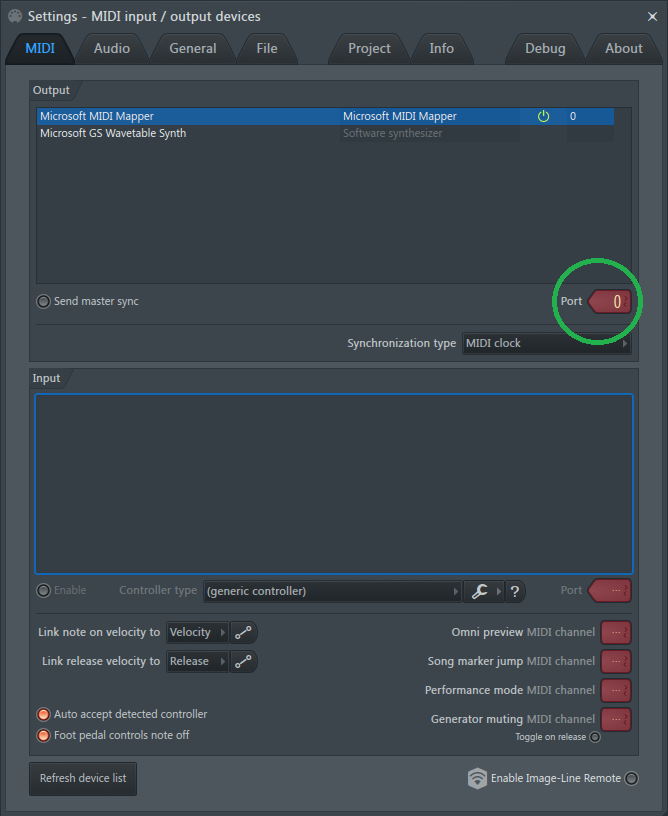
\includegraphics[width=.63\linewidth]{images/MIDIPort.png}
	\caption{MIDI Port wählen}
	\label{MIDIPort}
\end{figure}

Zusätzlich kann über den Reiter \textit{Project} die Timebase auf 48 PPQ eingestellt werden. Dadurch sind alle Noten und Pausen im richtigen Maß quantisiert, wodurch garantiert ist, dass die zeitliche Auflösung nie überschritten wird.

\bigskip

Ab jetzt sind alle Vorkehrungen getroffen und die MIDI Datei kann nach den bereits erwähnten Einschränkungen bearbeitet werden (pro Kanal nur eine Note gleichzeitig, maximal 8 Kanäle, Noten zwischen den Oktaven o1c bis o6a).
Zusätzlich sollte darauf geachtet werden, welche Noten in den Kanälen 7 und 8 liegen. Kanal 8 ist in SMW hauptsächlich für den Sprung Soundeffekt reserviert (und einige weitere die aber eher selten benutzt werden), Kanal 7 für die restlichen Soundeffekte. Das hat zur Folge, dass vor allem lange Noten und Noten, die für eine markante Melodie zuständig sind, nicht in diesen beiden Kanälen untergebracht werden sollten. Jedes mal wenn ein Soundeffekt in SMW abgespielt wird, werden die Noten des entsprechenden Kanals stumm geschaltet. \\
Die vollständigen Listen aller Soundeffekte befinden sich in den Ordnern 1DF9 (Kanal 7) und 1DFC (Kanal 8).

\bigskip

Entspricht die MIDI Datei den Anforderungen, sollte das Projekt als .mid exportiert werden falls man nicht die Trial Version von FL Studio besitzt, weil man keine Projektdateien öffnen kann, MIDI Dateien aber schon (wie wir offensichtlich gesehen haben). \\
Hier sei noch einmal gesagt, dass man darauf achten soll, nicht FLEX zu benutzen, da es passieren kann, dass die exportierte MIDI Datei keine Noteninformationen enthält und alle Arbeiten verloren gehen.

\subsection{Einführung FL Studio}

Ein vollständiges Tutorial zu FL Studio würde bei weitem den Rahmen sprengen, es werden jedoch auf die Grundfunktionen eingegangen die ausreichen, um MIDI Dateien zu bearbeiten. Abbildung \ref{FLStudio} zeigt das Programm in mehrere Abschnitten unterteilt. Dabei  handelt es sich um:


\begin{itemize}
	\item 1. Channel Rack
	\item 2. + 3. Playlist
	\item 4. Play/Pause
\end{itemize}


\begin{figure}[htbp] \centering
	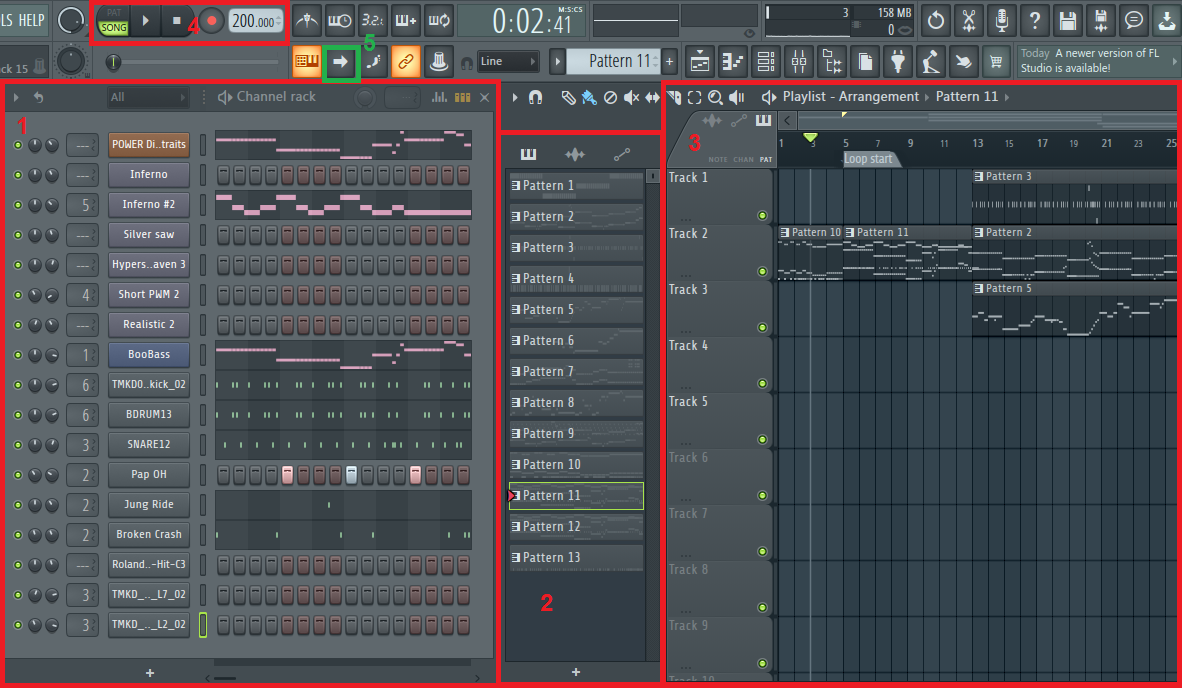
\includegraphics[width=.95\linewidth]{images/FLStudio.png}
	\caption{FL Studio Übersicht}
	\label{FLStudio}
\end{figure}

\subsubsection*{Channel Rack}

Im Channel Rack (F6) arbeiten wir die meiste Zeit. Hier befinden sich Kanäle, die entweder aus einem einfachen Sample oder einem VST (Virtual Studio Technology) Plugin bestehen. Jeder Kanal kann Noten beinhalten (im Falle eines Automation Clips ein Steuersignal). \\
Mit dem grünen Punkt links vor jedem Kanal kann dieser Stumm geschaltet werden. Der linke Regler ist für das Panning (Lautstärkeverteilung auf Lautsprechern) und der rechte für die Lautstärke des Kanals zuständig. Das Feld daneben kann mit einer Zahl besetzt werden. Diese gibt an, welchen Platz der Kanal im Mixer (F9) belegen soll, um dort weiter mit Effekten wie Reverb etc. bearbeitet zu werden. Da wir nur mit MIDI arbeiten, kann sowohl dieses Zahlenfeld, als auch der Mixer ignoriert werden. \\
Mit einem Linksklick auf einen Kanal öffnen wir diesen. Je nachdem, was sich dort befindet, öffnen sich entweder der Plugin Editor oder die Sample bzw. Instrument Settings. Mit einem Klick auf den kleinen Pfeil in der oberen linken Ecke öffnet sich ein Menü, worüber man bei Plugins  beispielsweise Presets (also Voreinstellungen) laden kann. (Im Falle von MIDI OUT können so voreingestellt CC's (Continuous Controller) von Synthesizern geladen werden. Wie man MIDI Controller auch selbst anlegt wird später erklärt.) \\
Klicken wir neben den kleinen Pfeil auf das Zahnradsymbol, öffnet sich eine weitere Leiste. Dort befinden sich neben dem grünen Mute Knopf, dem Panning und Volume Regler noch ein Pitch Regler (den wir u.a. für Pitch Slides ausnutzen können).

\bigskip

Mit einem Rechtsklick auf den Kanalnamen haben wir weitere Optionen. Die wichtigsten hierbei sind \textit{Insert} bzw. \textit{Replace}, womit ein Kanal ersetzt bzw hinzugefügt werden kann (Funktioniert auch über das + am unteren Rand des Channel Racks) und die Piano Roll (oder auch F7, wenn der Kanal ausgewählt wurde). In Abbildung \ref{Channel} ist dargestellt, wie ein neuer MIDI Out Kanal hinzugefügt werden kann.


\begin{figure}[htbp] \centering
	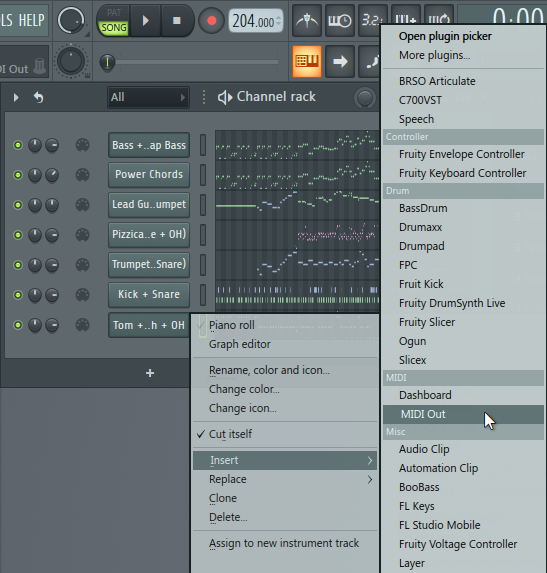
\includegraphics[width=.70\linewidth]{images/Channel.png}
	\caption{Channel einfügen}
	\label{Channel}
\end{figure}


Klickt man auf das schmale Select Feld (bekommt eine grüne Umrandung) ohne auf den Kanal geklickt zu haben (nicht dunkel unterlegt), kann mit der Tastenkombination Alt + Pfeiltasten ein Kanal verschoben werden.

\bigskip

Rechts neben dem Select Feld befindet sich der Step Sequencer bzw. eine Vorschau der Piano Roll. Mit den Standardeinstellungen hat der Step Sequencer einen 4/4 Takt, bestehend aus 16 16tel Noten. Den Step Sequencer verwendet man in der Regel nur mit Drum / Percussion Samples, da im Step Sequencer jede Note ein o5c ist. Die Piano Roll hingegen wird verwendet, um Noten in einen Kanal zu platzieren.

\subsubsection*{Playlist}

Als nächstes betrachten wir die Playlist. Der linke Bereich beinhaltet eine Liste an Pattern (Mustern), die im rechten Bereich der Playlist platziert werden können. In Abbildung \ref{FLStudio} besteht das Pattern 11 aus den Notenabfolgen, die im Channel Rack links daneben zu sehen sind. Wir können ein neues (leeres) Pattern über das + am unteren Fensterrand hinzufügen oder mit dem Feld Pattern über der Playlist (dort ist es auch möglich, ein Pattern zu kopieren, falls man ein ähnliches Muster haben möchte aber nur leicht bearbeitet werden soll)
Wir können so aus vielen kleinen Pattern Schnipseln einen Song bauen. \\
Es ist auch möglich, einen Song ohne Playlist zu bauen, indem sich der gesamte Song in nur einem Pattern befindet (was automatisch der Fall ist, wenn man eine MIDI Datei mit FL Studio öffnet).

\bigskip

In Feld 4 befinden sich die Play/Pause, Stop und Aufnahme Buttons. Außerdem kann über \textit{PAT} (orange) bzw \textit{SONG} (grün) bestimmt werden, ob das ausgewählte Pattern oder die Playlist abgespielt werden soll. \\
Rechts daneben befindet sich die BPM Anzeige, die das Tempo bestimmt. Mit einem Rechtsklick auf diese kann über den Punkt \textit{Tap} im Rhythmus eines Songs getippt werden, um die BPM Zahl einfach zu bestimmen. \\

Mit dem in Abbildung \ref{FLStudio} grün markierten Feld 5 schaltet man das automatische scrollen während des Play Vorgangs ein bzw. aus. Ich bevorzuge kein Autoscroll.

\subsubsection*{Piano Roll}

Werfen wir einen Blick auf die Piano Roll, können wir diese auch in mehrere Bereiche aufteilen. Im Hauptbereich können wir Noten platzieren und diese von der Länge anpassen, indem man am rechten Rand einer Note zieht (kann auch umgestellt werden). \\
Die senkrechten Striche im unteren Bereich geben die Lautstärke jeder einzelnen Note an. Diese kann dort verändert werden, es kann auch über das Feld \textit{Control} zwischen unterschiedlichen Parametern gewechselt werden (z.B. Panning). \\
Oben links in der Ecke befindet sich ein Pfeil, der eine Menge nützlicher Einstellmöglichkeiten
beinhaltet. Die wichtigsten sind \textit{Snap}, womit bestimmt wird, mit welchem Inkrement Notenlängen geändert und Note platziert werden und die \textit{Quantize} Funktionen unter Tools, womit markierte Noten auf eine vorgegebene Auflösung quantisiert werden können.

%\newpage

\begin{figure}[htbp] \centering
	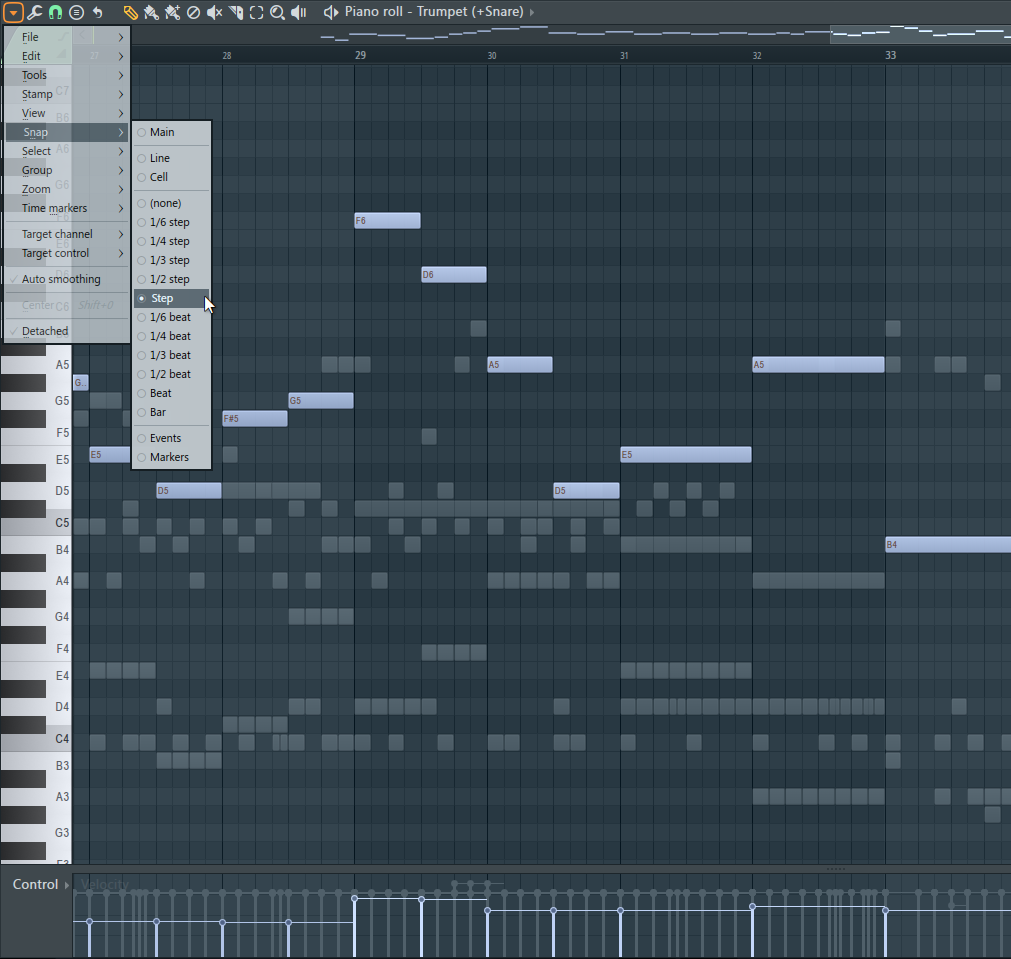
\includegraphics[width=.95\linewidth]{images/PianoRoll.png}
	\caption{Piano Roll Optionen}
	\label{PianoRoll}
\end{figure}

\bigskip

\subsubsection*{MIDI Out}

Erstellen wir einen MIDI Out Kanal wie in Abbildung \ref{Channel} und klicken auf den Kanal sehen wir die Plugin Settings. Die Channel Nummer ist das Äquivalent eines Kanals in MML, wobei die meisten MIDI/MML Konverter der Reihe und nicht nach Kanalnummer konvertieren. Eine Besonderheit ist der Kanal 10, dadurch wird die Piano Roll für diesen Kanal zu einem Drum Set, d.h. jede Note entspricht einem Drum bzw. Percussion Instrument. Rechts daneben kann im Feld \textit{Patch} ein MIDI Instrument für diesen Kanal ausgewählt werden. \\
Die Bank Felder können wir ignorieren, da wir keine Soundbanken verwenden werden. \\
Die Port Nummer muss die gleiche wie in Abbildung \ref{MIDIPort} sein, ansonsten fehlt die Soundausgabe.

\begin{figure}[htbp] \centering
	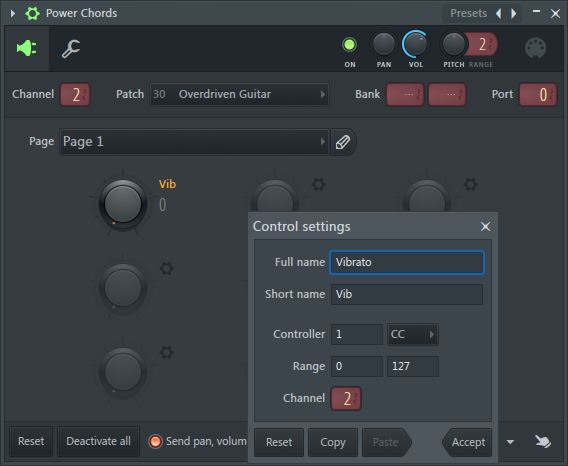
\includegraphics[width=.75\linewidth]{images/MIDIOut.png}
	\caption{geöffneter MIDI Out Kanal}
	\label{MIDIOut}
\end{figure}

Unten befindet sich ein Bereich mit 9 Reglern. Diese sind zunächst ohne Funktion, können von uns aber mit Controllern belegt werden. Dafür muss man mit einem Rechsklick auf das kleine Zahnrad neben dem Regler klicken um die Control Settings zu öffnen. \\
Hier kann man jedem Regler einen Namen und Funktion zuordnen. Wir benutzen Continuous Controller (CC) die je nach Nummer eine andere Funktion abdecken. Eine vollständige Liste der CC Nummern gibt es unter: \\ \href{https://nickfever.com/Music/midi-cc-list}{https://nickfever.com/Music/midi-cc-list} \\
CC Nummer 1 ist beispielsweise ein Controller für Vibrato. Die Range bestimmt einen Wertebereich, den man i.d.R. bei 0 bis 127 lassen sollte. \\
Die Letzte Channel Angabe bestimmt, welche Kanäle man mit genau diesem Regler ansteuern möchte.

\bigskip

An dieser Stelle sei gesagt, dass nicht alle CC's über MIDI Out selbst funktionieren (generell unterstützt nicht jedes Plugin oder Synthesizer alle Controller). Außerdem werden die Controller nicht mit in den MML Code konvertiert, sie sind aber dennoch hilfreich als Referenz.

\bigskip

Ein nützliches Plugin ist BRSO Articulate, zu finden unter: \\ \href{https://www.syntheticorchestra.com/tools/articulate/}{https://www.syntheticorchestra.com/tools/articulate/} welches das MIDI Out Plugin von FL Studio ersetzt. Das Plugin kann sich selbst mit mehr Controllern ansteuern und es können Instrumente abhängig von der Farbe einer Note gesetzt werden (Noten Farben können in der Piano Roll geändert werden). Eine ausführliche Anleitung zum Plugin findet sich auf der Webseite. \\
VST Plugins lassen sich in FL Studio installieren, indem man die entsprechende .dll Datei des Plugins in den Ordner \textit{Plugins/VST/} oder \textit{Plugins/Fruity/Generators} legt und dann in FL Studio diese über die Plugin Database (links) aktiviert nachdem man sie über \textit{Options/Manage Plugins} gesucht hat.

\bigskip

Falls man nur die Trial Version von FL Studio besitzt und man keine Projekte öffnen kann, sind die Einsatzmöglichkeiten von BRSO Articulate begrenzt (genau auf eine Session).